\chapter{Implementation of Applications}
Store the current order of product and its meta information, find the which shelf stores the current requested product, assign an idling logistic unit to pick up the itinerary ... I/O operations make up the majority of SAP business scenarios. 
 In the load test conducted in this paper, applications are built to realize a scenario: advertisements are published in a bulletin board and clients can browse through the items. 

The PostgreSQL backing service from Cloud Foundry is used as database. As the goal is to test how the application handles large amount of concurrency instead of the database efficiency, data will not be queried in high quantity or complicated joined actions  in the test. 

To bring Java and node.js to a comparable level, the applications are implemented with minimum use of frameworks so that the overhead or any other influential factors on performance can be first taken off the table. 
\section{Java implementation}
\missingfigure{Add figure for java application implementation}

\begin{figure}[h]
	\centering
	\includegraphics[width=12cm]{java-structure}
	\caption{java application implementatio}
	\label{java-implementation}
\end{figure}

Figure \ref{java-implementation} shows the implementation of the Java application. It uses embedded Jetty server to handle plain HTTP requests. No REST or any other kind of web services is implemented. The connection with database is plain JDBC. CRUD operations are implemented with query statements. No ORM is utilized. Since the data structure is intentionally kept simple: only one table and with no complex data types, the application without ORM is quite in order.\\
\section{optimize the Java implementation}
All possible attempts are made to bring about every potential performance of the application. Since there is no complex logic, the focus of optimization lays on the interaction between applications and database. In case of Java implementations, to set a optimal thread pool configuration is also investigated. \\
The first checkpoint is database connection which greatly affect performance since it is the most expensive operation in the application which has no complicated computing logic. Opening a connection and closing it with every request would gigantically slow down the application. Therefore connection pool is a key component in the implementation. It turns out there are quite a few libraries which handles connection pooling. In the thesis,  three different libraries are tried out. \textit{PGPoolingDataSource}  \citep{pgpool}   comes with default PostgreSQL JDBC driver. \textit{commons-dbcp2} \citep{dbcp} package from Apache Software Foundation provides an opportunity to coordinate the efforts required to create and maintain an efficient, feature-rich package under the \ac{ASF} license. \textit{HikariCP} is a "zero-overhead" production ready connection pool. It turns out \textit{HikariCP} \citep{hikari} has outperformed the other two. \\
The next thing is to find an ideal configuration for the connection pool size. In an article from Brett Wooldridge \citep{hikari}, it is pointed out larger connection pool size configuration doesn't necessarily lead to a better performance. Single core can only execute one thread at a time; then the OS switches contexts and that core executes code for another thread, and so on. It is a basic Law of Computing that given a single CPU resource, executing A and B sequentially will always be faster than executing A and B "simultaneously" through time-slicing. However, there are a few other factors at play. For example, databases typically store data on a disk, which traditionally is comprised of spinning plates of metal with read/write heads mounted on a stepper-motor driven arm. So there is a time cost for disk "I/O wait".  During this time that the OS could put that CPU resource to better use by executing some more code for another thread. So, because threads become blocked on I/O,  more work can be done by having a number of connections/threads that is greater than the number of physical computing cores. In the case of thesis, database is running in Diego cell which contains 4 CPUs. In order to verify and find the best fit for the load the thesis intend to generate, an experiment is conducted with connection pool size of 30, 60, and 90.  Figure \ref{pool-comparison}, shows a slight difference can be deducted that the pool size of 90 reaches the upper limit of total transaction slightly earlier than the other configurations. Slightly better is the performance from a connection pool size of 60 than that of 30.

\begin{figure}[h]
	\centering
	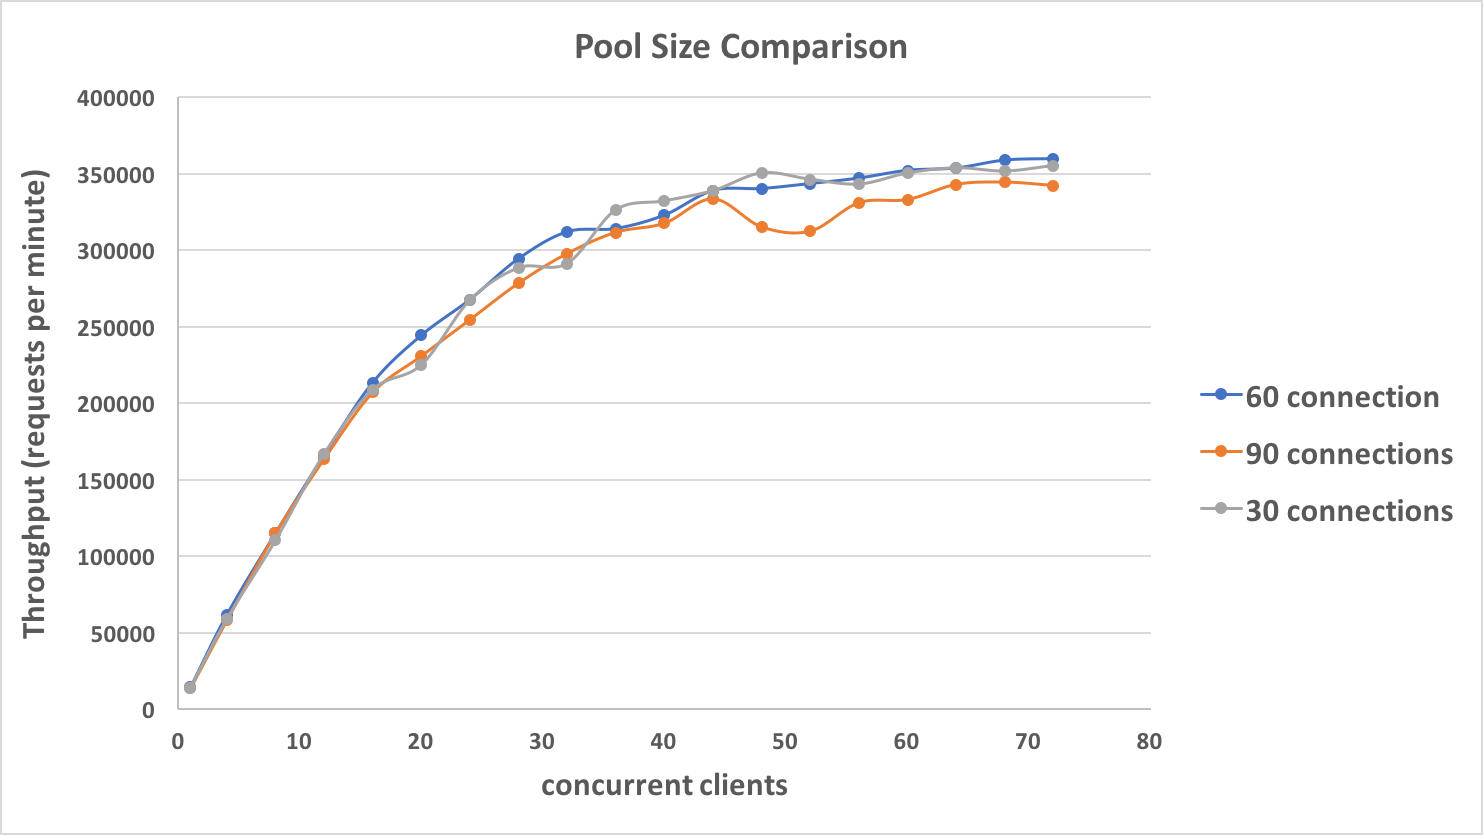
\includegraphics[width=12cm]{pool_size_con_user}
	\caption{Database connection pool size comparison}
	\label{pool-comparison}
\end{figure}

Thread pool size is also scrutinized and following the recommendation made by Jetty \citep{threadpool}, the size is set from 10 to 400. \\

 \section{Node.js implementation}
 \missingfigure{Add figure for java application implementation}
 
 \begin{figure}[h]
 	\centering
 	\includegraphics[width=12cm]{java-structure}
 	\caption{node application implementatio}
 	\label{node-implementation}
 \end{figure}
 
Figure \ref{node-implementation} shows the implementation of node application. It uses the standard node.js library to build the web platform. One other dependency it has is the database connection. 

\section{optimize the node.js implementation}
Node.js application basically faces the same configuration of connection pool in database. In the thesis, also three different libraries are tried out. Unlike Java libraries, there is some overlapping in regard to the node libraries. In npm, one can find a number of PostgreSQL drivers. However, majority of them are built on the basis of one library: "node-postgres/pg" \citep{node-pg}. They are either wrappers or additional implementation with "promise" or "async/wait". For example, a great difference can not be derived from using of "node-postgres/pg" and "pg-promise" in the scenario in this thesis. The comprehensive research on framework benchmarking \citep{benchmark} uses "Sequelize", which is also tried out in the thesis. However, it yields even a worse performance result because the object mapping costs indisputably computing time. In the end, the suggestion from "node-postgres/pg" writer is adopted to use "pg-native" which can boost a 20-30\% increase in parsing speed. There is not much varieties of pooling in node either. "node-postgres/pg" uses "pg-pool" which again utilizes "generic-pool". In the thesis, they are all checked out, but no significant difference is found. Therefore, the implementation of Node.js application sticks to "node-postgres/pg" and uses the built in connection pool.\\




